\newpage
\section{Evaluation and results}
\label{sec:evaluation}
Throughout this thesis, a few experiments were conducted to evaluate the performance of the trained model in terms of quality of the generated images. The results of these experiments have been consolidated in this section.\\
To assess the quality of conditional image synthesis, a survey was prepared, comprising 20 distinct sketches, each associated with four images. Among the four images, one was generated from the sketch, while the other three were selected from the FFHQ dataset based on the similarity metric described in~\ref{sec:xcos}. The FFHQ dataset has been chosen due to the fact that it was the dataset used to train the model. The 20 images were chosen from 3256 sketches done by people during a scientific research festival on a graphic tablet. These sketches were made on the graphical interface described in~\ref{sec:testing setup}.\\
In the process of collecting the sketches, it was observed that if the size of the sketches was too small or if the position of the eyes was too high or low on the graphical interface, the resulting generated image did not accurately resemble the original sketch. To address this issue, two horizontal lines and a vertical line, discussed in section \ref{sec:testing setup}, were added. This allowed individuals to have a better understanding of the appropriate size of the sketch and the correct placement of the main facial characteristics to ensure accurate image generation. Furthermore, it has been observed that the sketches made using a pen with a thickness greater than three tend to result in bad images, despite the talent of the artist who created the sketch.\\
Fig. \ref{fig:disappointing sketch small} shows an instance of unsatisfactory outcome achieved from a highly realistic sketch, which was produced using a very small scale.
%or with a pen that was excessively thick.
\begin{figure}[htbp]
  \centering
  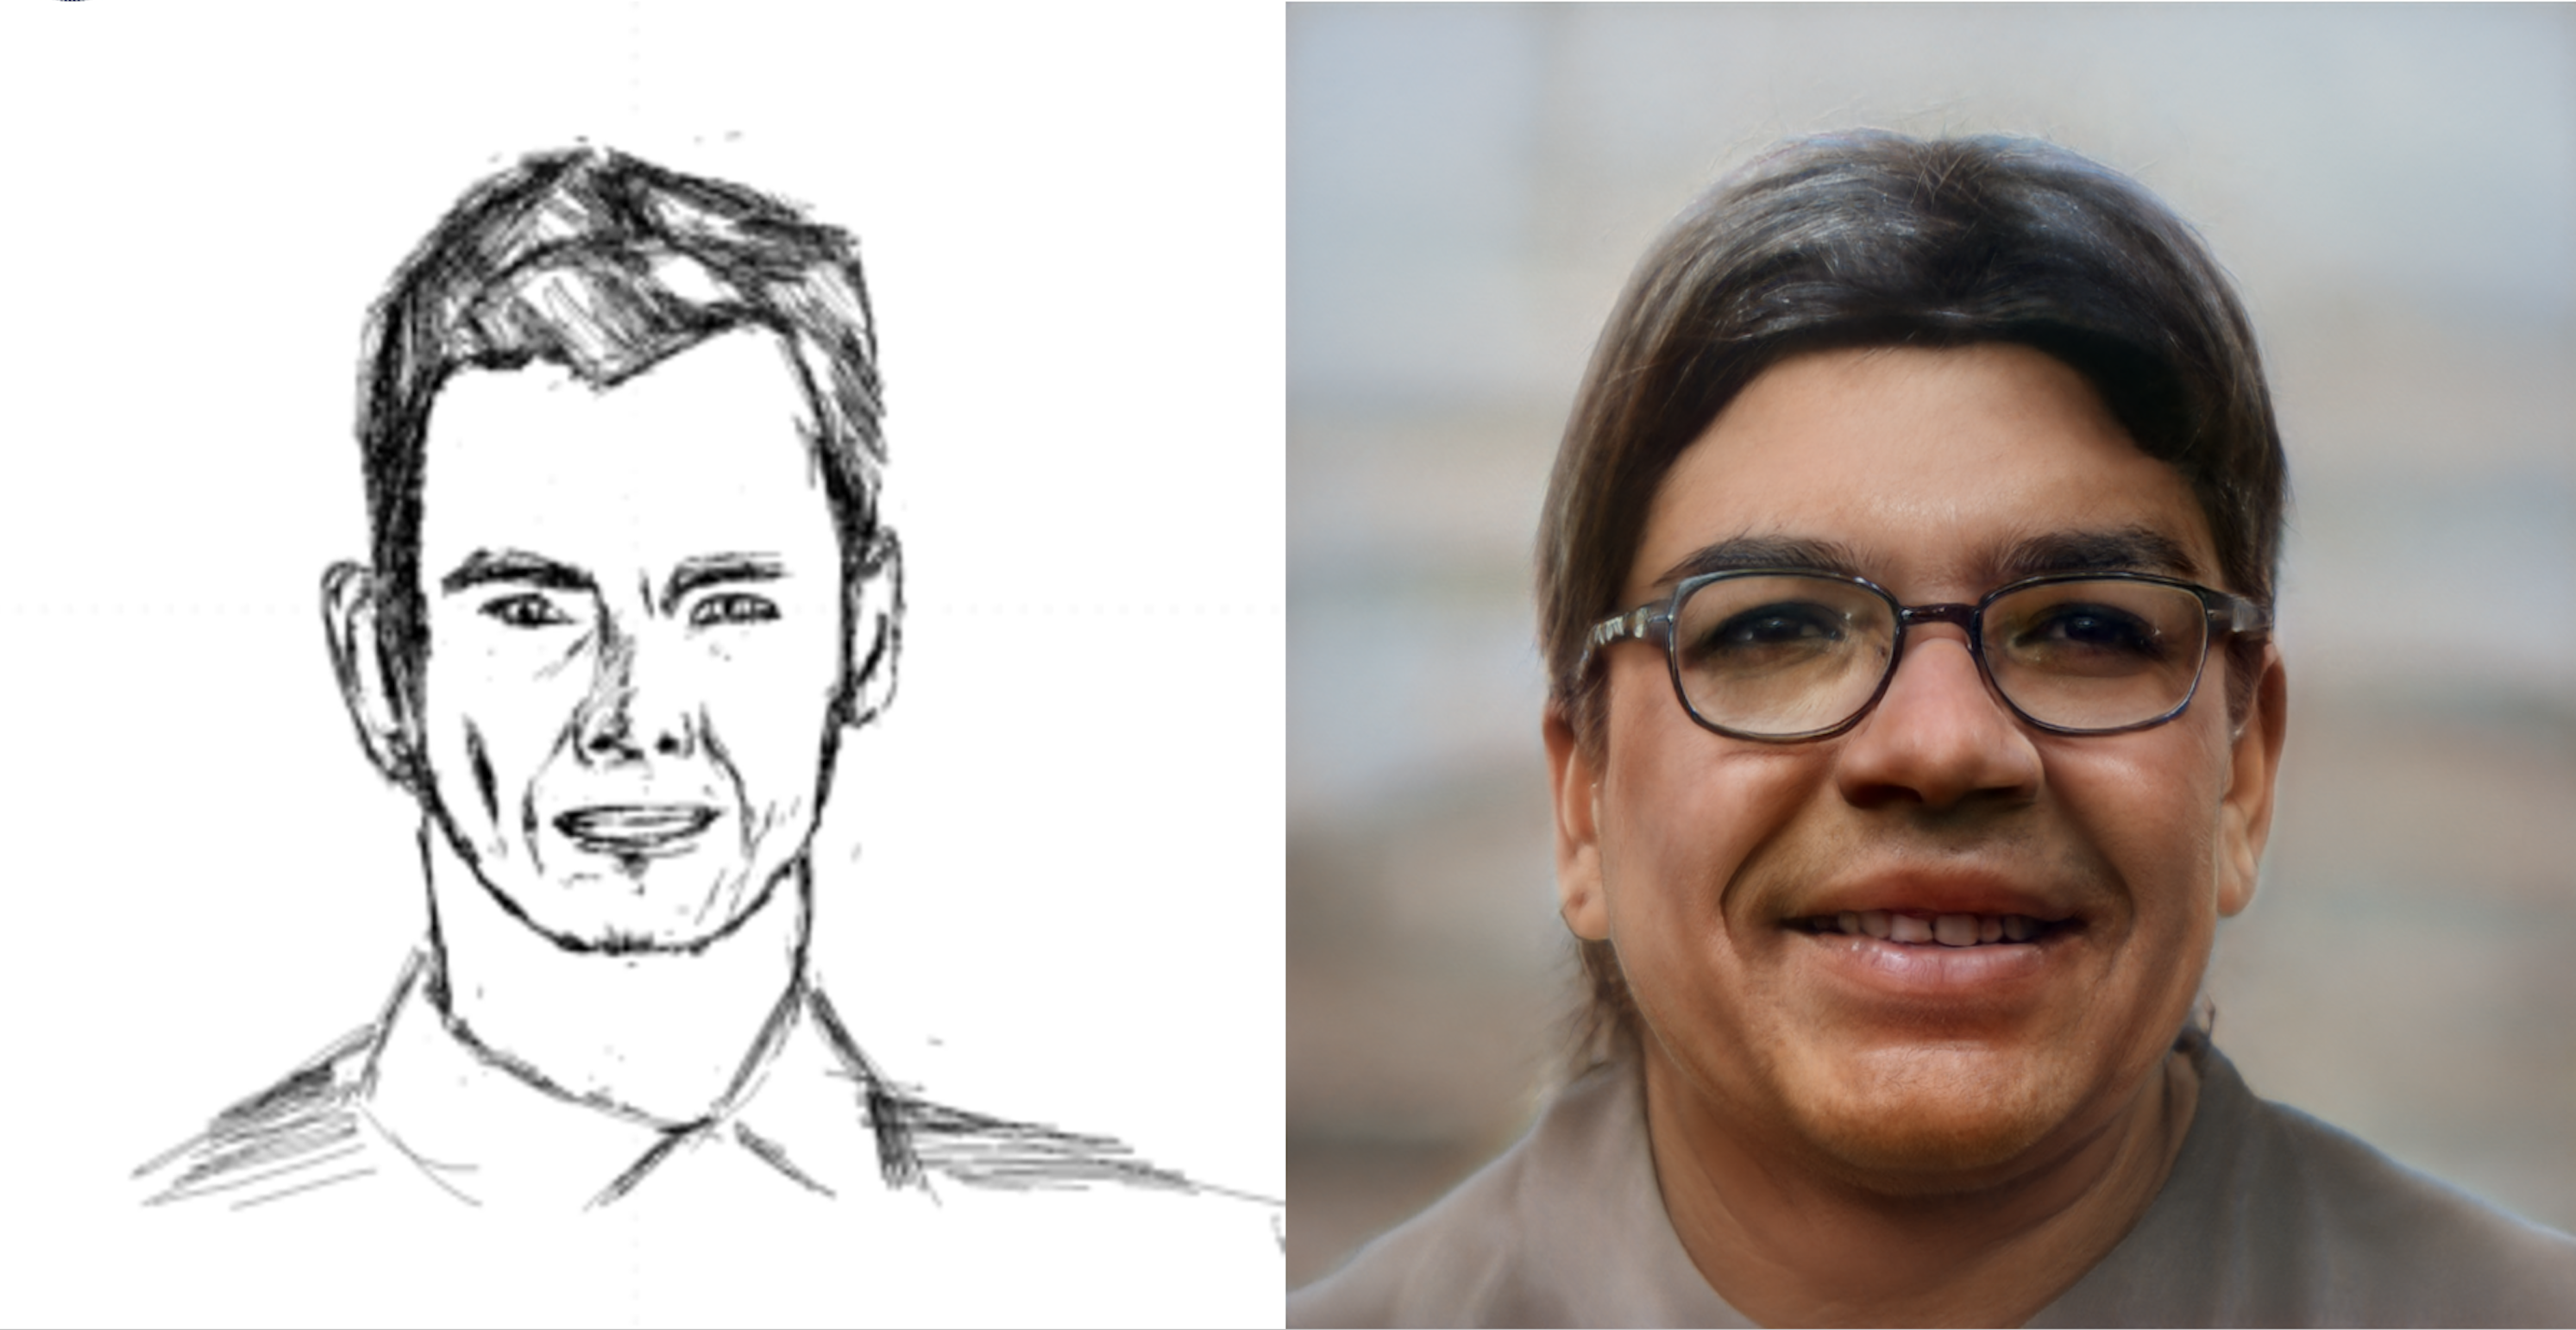
\includegraphics[scale=0.15]{figures/badResult1.png}
  \caption{Disappointing result generated from a sketch too small}
  \label{fig:disappointing sketch small}
\end{figure}

\noindent As illustrated in Fig.~\ref{fig:result thick pen}, the use of a pen too thick can have a negative effect on the generated images, for example it can generate unrealistic hair. However, upon closer examination of the generated image, it can be observed that certain details of the original sketch are still present. 
\begin{figure}[htbp]
  \centering
  \includegraphics[scale=0.15]{figures/badResult.png}
  \caption{Result obtained from a sketch made with a thick pen}
  \label{fig:result thick pen}
\end{figure}
%

\noindent Impressive results can be achieved when the sketch is created by a skilled person with a proper size using a pen of suitable thickness. It is worth noting that the success of the generated image is highly dependent on the quality of the input sketch. Where the term “quality” is related to the dimension of the sketch and the pen's thickness.
Therefore, it is essential to carefully consider the conditions under which the sketch is created to obtain optimal results. An example of a very breathtaking result can be seen in Fig.~\ref{fig:impressive result}, while Fig.~\ref{fig:result simple sketch} depicts a straightforward input sketch and its corresponding generated image that exhibits noticeable similarity.
\begin{figure}[htbp]
  \centering
  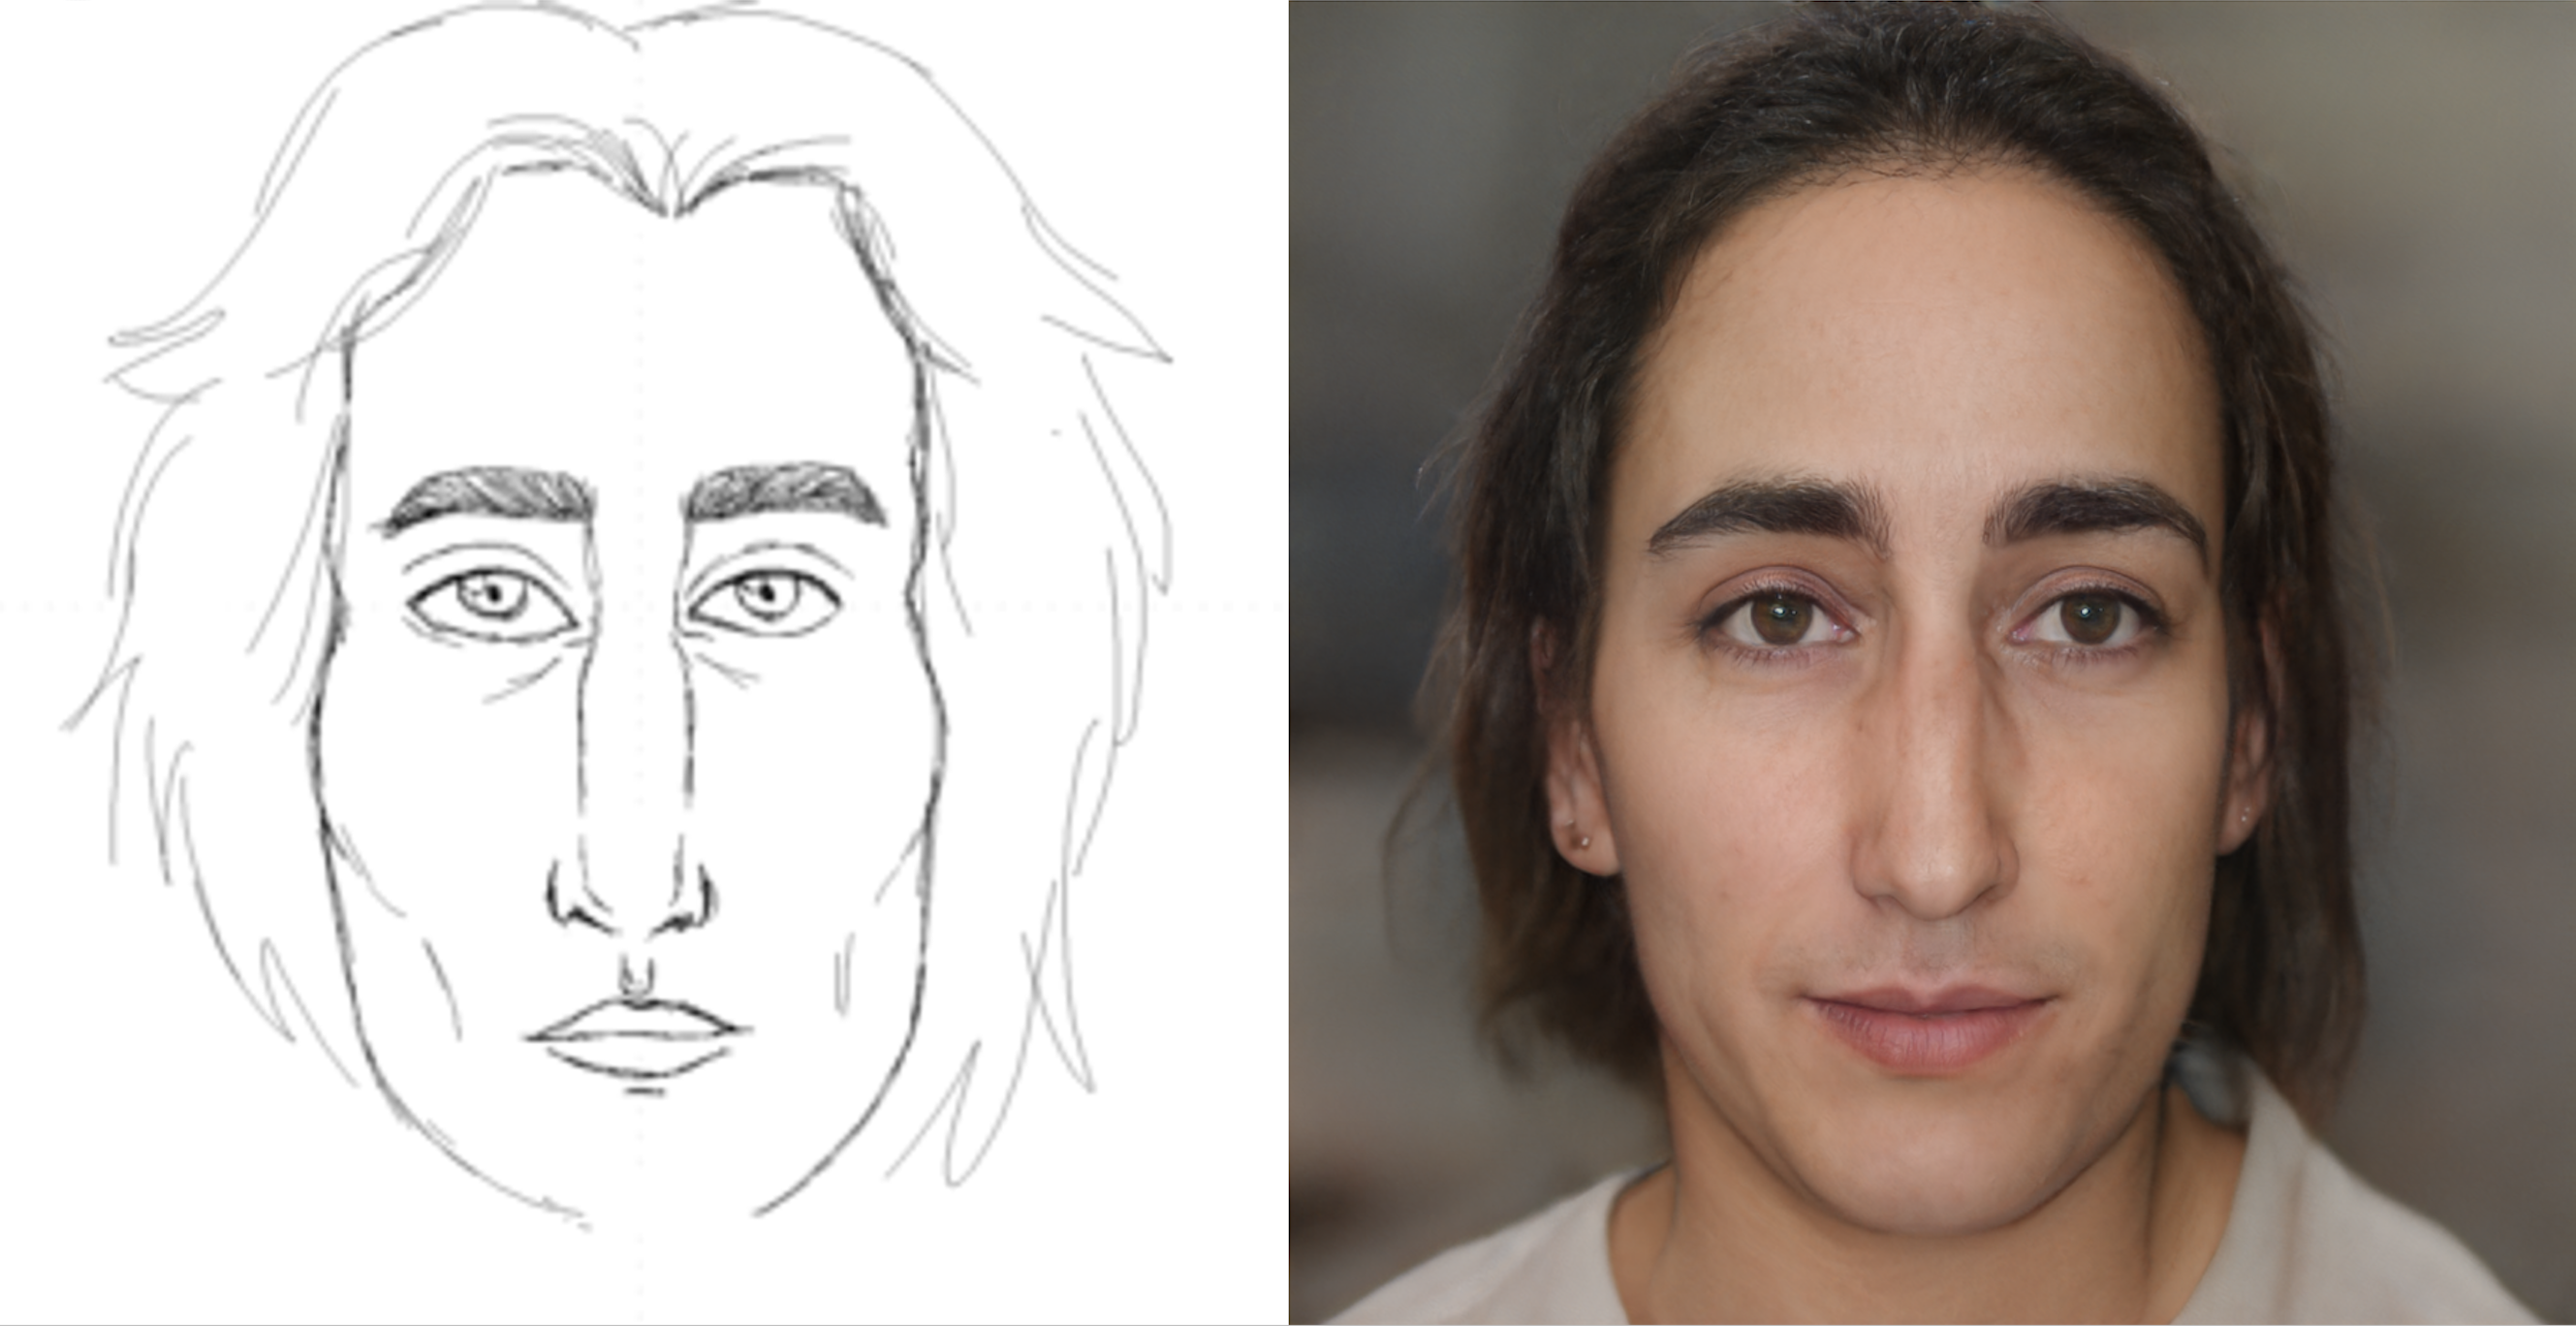
\includegraphics[scale=0.15]{figures/goodResult.png}
  \caption{Impressive result of an image generated from a sketch}
  \label{fig:impressive result}
\end{figure}
\begin{figure}[htbp]
  \centering
  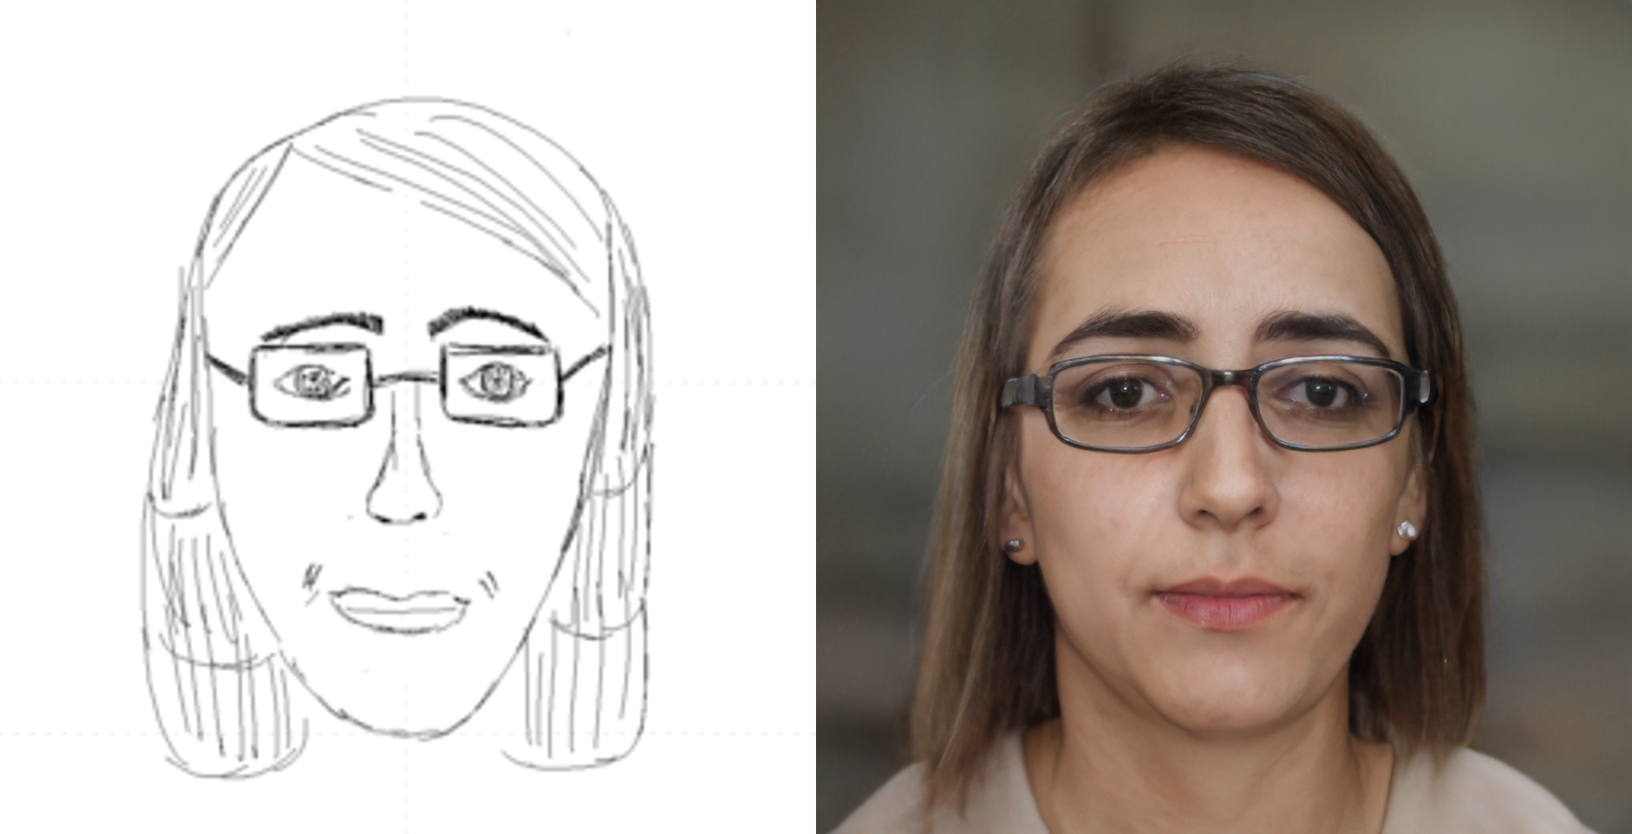
\includegraphics[scale=0.25]{figures/goodResult-simpleSketch.png}
  \caption{Result of an image generated from a simple sketch}
  \label{fig:result simple sketch}
\end{figure}
%

\noindent Due to the diverse range of people who contributed to the sketch dataset, encompassing varying age groups and drawing abilities, it was necessary to filter out unrealistic sketches. Furthermore, some sketches displayed minor differences, as shown in Fig. \colorbox{yellow}{AGGIUNGERE IMMAGINE}, or only portrayed the outline of the face without any distinguishable features (Fig.~\ref{fig:discarded images}).
\begin{figure}[htbp]
    \centering
    \subfloat[][\emph{Empty sketch}]
    {
\includegraphics[width=.4\textwidth]{figures/emptySketch.png}} \quad
    \subfloat[][\emph{Sketch with just the contour of the face}]
    {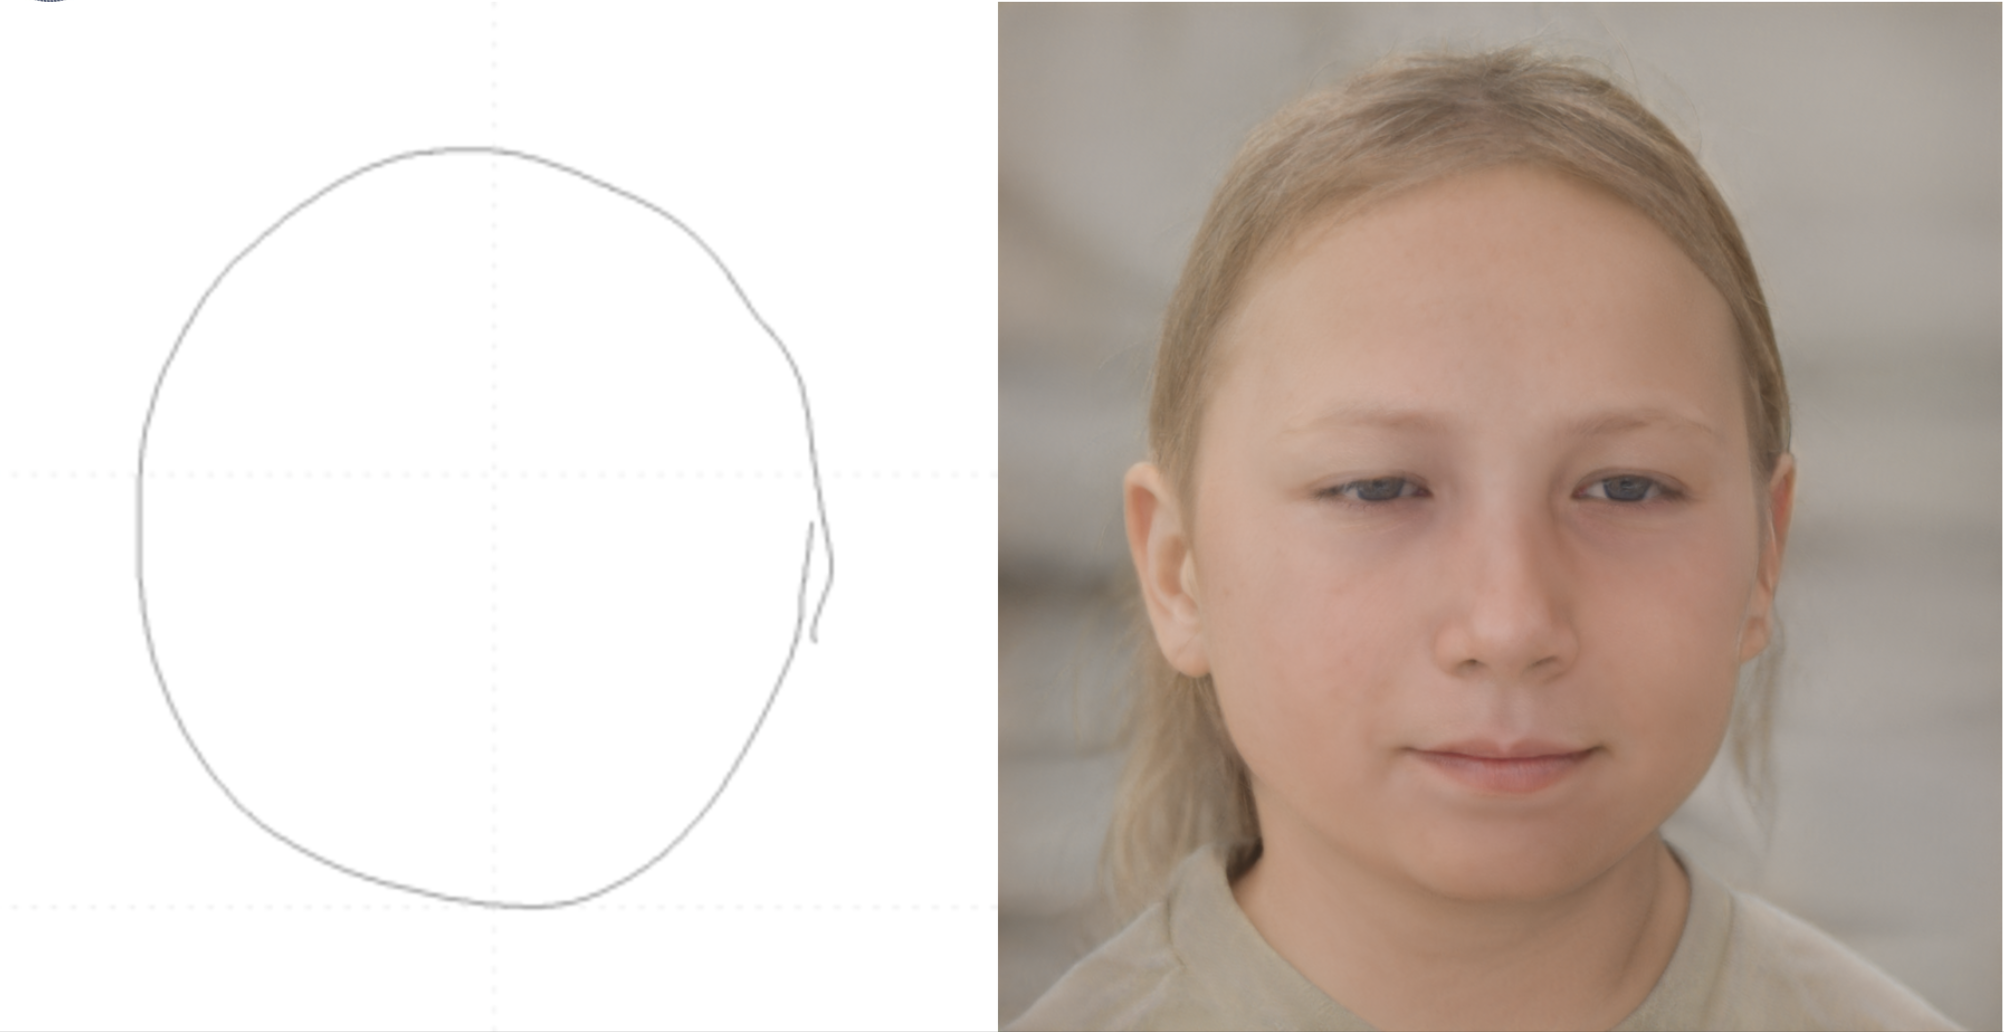
\includegraphics[width=.4\textwidth]{figures/sketchOnlyContour.png}}\\
    \caption{Examples of discarder images}
    \label{fig:discarded images}
\end{figure}
Therefore, the initial set of sketches was manually processed to remove such sketches, leaving only the more realistic ones. Subsequently, the remaining images underwent further analysis, and the poorest sketches were discarded. Finally, the xCos metric was applied to the filtered dataset to identify the most similar images to the sketch.\\ \\
%
%
%
The survey was built in such a way that 5 random images out of the 20 are displayed. The survey's participants were instructed to choose the image that in their opinion had inspired the realisation of the sketch. An example of an image displayed in the survey is shown in Fig.\colorbox{yellow}{da aggiungere}
\\
\colorbox{yellow}{QUANDO AVRò I DATI METTO QUA I RISULTATI}
%
%
%

% PER QUANDO AVRò I DATI VEDERE SE POSSO INCLUDERE QUESTE FRASI
%The data obtained from the survey were analysed using descriptive statistics to determine the mean ratings for each of the criteria. The analysis of the survey data provided valuable insights into the quality of the generated images and their similarity to the images from the FFHQ dataset. The open-ended questions were also analyzed to provide qualitative insights into the participants' perceptions of the quality of the generated images.

%In summary, the survey design was carefully crafted to evaluate the quality of conditional image synthesis by comparing the generated images with visually similar images from the FFHQ dataset. The results of the survey can be used to guide future research in conditional image synthesis techniques and can serve as a benchmark for the quality of generated images.